%%%%%%%%%%%%%%%%%%%%%%%%%%%%%%%%%%%%%%%%%%%%%%%%%%%%%%%%%%%%%%%%%%%%%%%%%%%%%%%
\section{The physics of magnetic monopoles}
\label{sec:theory}
%%%%%%%%%%%%%%%%%%%%%%%%%%%%%%%%%%%%%%%%%%%%%%%%%%%%%%%%%%%%%%%%%%%%%%%%%%%%%%%
To date there has been no solid, reproducible experimental evidence that
magnetic monopoles exist. For now, magnetic charge remains an entirely
theoretical concept that would, amongst other things, neaten up Maxwell's
equations of electrodynamics.
%
So why would we -- \emph{why should we} -- spend time and effort looking
for them? There are, in fact, some very good reasons to believe they exist
and that we just haven't found them yet.
%
One theorist has even said that they are ``\emph{one of the safest
bets one can make about physics not yet seen}''~\cite{Polchinski2004}.
%
In this section we look at some of these reasons -- so you
can decide for yourself!

%=============================================================================
\subsection{Dirac's magnetic monopole}
\label{sec:diracmonopole}
%=============================================================================
Paul Adrien Maurice Dirac (Figure~\ref{fig:pamdirac}) was a theoretical
theorist who played an important part in the development of quantum mechanics.
He was one of the first theoreticians to combine quantum mechanics with
special relativity with his eponymous equation~\cite{Dirac1928},
which allowed so-called ``negative energy'' solutions~\cite{Dirac1930}.
%
At first Dirac interpreted these solutions,
which would require the particle corresponding to the negatively-charged
electron to have a positive charge, as protons.
%
He noted in a subsequent paper~\cite{Dirac1931} that, actually,
the negative energy particles would need to have the same mass as the
electron -- the positively-charged anti-electron.
%
He had predicted antimatter.
%
This prediction was confirmed with Anderson's discovery of the
positron~\cite{Anderson1933} and the rest, as they say, is history.

%
\begin{figure}[htbp]
  \centering
  \includegraphics[width=0.25\textwidth]{assets/images/dirac-portrait/paul-dirac_nobel1933.jpg}
  \caption[Paul A. M. Dirac]
  {\label{fig:pamdirac}%
Paul Adrien Maurice Dirac (1902-1984) predicted the existence of antimatter~\cite{Dirac1930}.
Could he have been right about magnetic monopoles too?~\cite{Dirac1931}.
Image credit: nobelprize.org (public domain); please refer to their website
regarding re-use of this image.} 
\end{figure}
%

Funnily enough, in the same paper Dirac had made another prediction.
(In fact, this prediction was the main point of the paper!)
In trying to explain why there was a smallest, discrete value of the
electric charge (i.e. why charge is quantised),
he postulated the existence of isolated magnetic charge that would show
a ``\emph{symmetry between electricity and magnetism quite foreign to current views}''.
He had predicted the magnetic monopole.

%
\begin{figure}[htbp]
  \centering
  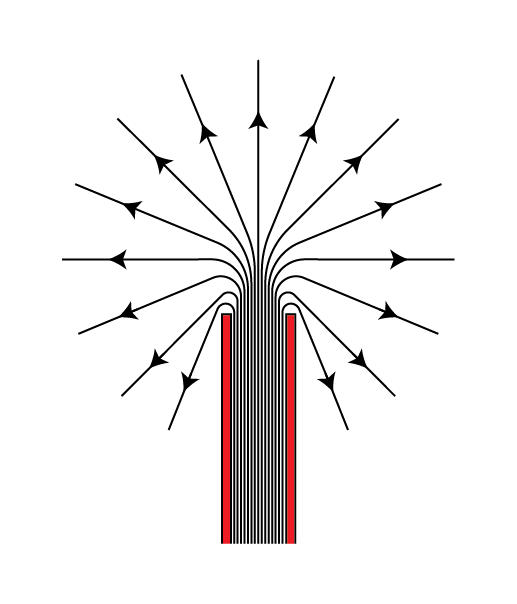
\includegraphics[width=0.5\textwidth]{assets/images/dirac-monopole/dirac-monopole.png}
  \caption[A schematic representation of Dirac's magnetic monopole]
  {\label{fig:diracmonopole}%
A schematic representation of Dirac's magnetic monopole.
The monopole is imagined to be the end point of a semi-infinitely long,
infinitesimally thin solenoid known as a ``Dirac string'',
here shown from the side (red lines).
%
The magnetic field lines (black arrows) are shown emanating from the point
at the end of the string (imagine the red lines are infinitely close together).
If such Dirac monopoles exist, it is the requirement that the string is
undetectable that means electric charge must be quantised.
%
Image credit: \href{http://researchinschools.org}{Institute for Research in Schools}.}
\end{figure}
%

Dirac's monopole was bit of a funny object.
Like a particle with electric charge,
the monopole would need to exude magnetic field field lines spherically
from its centre. Other magnetic charges placed in this field would experience
a force exactly analogous to the Coulomb force that pushes like charges apart
and pulls opposite charges together.
To create such a magnetic field configuration,
Dirac imagined a semi-infinitely long, infinitesimally thin solenoid
(i.e. a very, very tightly-wound coil with a flowing electric current).
%
The end of this ``Dirac string'' -- as shown schematically in
Figure~\ref{fig:diracmonopole} 2 -- represents the monopole.

While it is easy to imagine such a string,
one might not necessarily want to get tangled up in it.
Dirac showed that if such a string/monopole configuration did exist in
Nature, the only way that the mathematics could work out such that the
strings were undetectable by experiments was if electric charge was quantised.
There is an excellent explanation of the quantum theory behind this assertion
using the double slit experiment (as well as many other aspects of magnetic
monopoles) in~\cite{Rajantie2012}.
%
As the quantisation of charge is observed experimentally,
Dirac reasoned that magnetic monopoles (and their associated strings)
must exist.
%
Unfortunately, unlike the positron, monopoles were not found a few years
later.

%=============================================================================
\subsection{Grand Unified Theories}
\label{sec:guts}
%=============================================================================
Theorists, in the meantime, had been developing \ac{QFT}
as a way of describing matter and forces not in terms of particles or waves 
but mathematical constructs called fields.
%
(If you want to get your head around the wave-particle duality,
study physics at university and take a \ac{QFT} course.
Your hands will thank you from all of the ``hand-waving'' you won’t have to do.)
%
The 1960s saw the electromagnetic and weak forces -- two of the fundamental
forces of Nature -- united into a single electroweak force,
winning Glashow, Salam and Weinberg the 1979 Nobel Prize for
Physics.
The 1970s then saw a great deal of interest in literally going one
better -- uniting the electromagnetic, weak, and strong forces into one force.
Such a theory is known as a \ac{GUT}. %Grand Unified Theories (GUTs).
Figure~\ref{fig:forceunification} shows roughly where this ``Grand Unification''
might occur in terms of energy (around $10^{13}$ \ac{TeV}) and time
(about $10^{-36}$ seconds after the Big Bang).

%
\begin{figure}[htbp]
  \centering
  \includegraphics[width=0.6\textwidth]{assets/images/force-unification/OT0082M.jpg}
  \caption[The unification of the four fundamental forces of Nature]
  {\label{fig:forceunification}%
The unification of the four fundamental forces of Nature,
as shown in this ``\emph{Postcard from the Terascale}''.
Image credit: Symmetry Magazine/Sandbox Illustrations; please contact them
regarding licensing/re-use of this image.}
\end{figure}
%

What does this have to do with magnetic monopoles?
Well, in the course of trying to get the mathematics to work,
two theorists independently found that an inevitable consequence of bringing
the three forces together was the appearance of terms in the equations that
represented particles (well, fields) with
magnetic charge~\cite{tHooft1974,Polyakov1974}.
You couldn't unite the strong force with the electroweak force
without magnetic monopoles\footnote{%
As it happens, the monopoles appear when you squeeze the \ac{GUT} to
quantise the electromagnetic field into particles.
So, as noted in many reviews of the magnetic monopole literature,
Dirac’s argument is reversed: the quantisation of the electromagnetic
field necessitates the existence of magnetic monopoles.}.
%
Of course, no Grand Unified Theory has been experimentally verified,
but if we believe in the ultimate unification of the
fundamental forces -- which, let’s be honest, would be rather nice -- it
turns out that we \emph{need} magnetic monopoles.

%=============================================================================
\subsection{Monopoles in the Standard Model}
\label{sec:smmonopole}
%=============================================================================
There is, however, one slight problem with \ac{GUT}-scale magnetic monopoles.
While one cannot predict the mass of the Dirac monopole,
\ac{GUT} monopole masses (which can be calculated) tend to be billions
and billions times the energies reachable by the \ac{LHC}, or indeed any
physical process occurring more than a fraction of a second after the Big Bang.
While we can look for ``relic'' monopoles in cosmic rays that reach the
Earth --and~\cite{Patrizii2015} provides an excellent summary of the searches
conducted so far -- we would need something between the Dirac monopole
and the \ac{GUT} monopole in order to have some hope of creating
magnetic monopoles in accelerators with all of the benefits that the
controlled conditions of the laboratory bring.

%
\begin{figure}[htbp]
  \centering
  \includegraphics[width=1.0\textwidth]{assets/images/monopole-artist/moedal_2048_landscape.png}
  \caption[An artist's impression of magnetic monopole production at the LHC]
  {\label{fig:monopoleartist}%
An artist's impression of magnetic monopole production in a proton-proton
collision at the \acf{LHC}. Image credit: The MoEDAL Collaboration/H. Valja 2015;
please contact them regarding licensing/re-use of this image.}
\end{figure}
%

Fortunately, such a monopole has been proposed.
An ``\term{electroweak monopole}'' (which, incidentally, has twice the
magnetic charge of Dirac's monopole) can be made to appear in the
Standard Model of particle physics by adding some extra terms to the
field equations~\cite{Cho1997,Yang1998}.
In fact, the theorists behind the electroweak monopole insist that the
Standard Model is incomplete without the electroweak monopole -- and
given that we know the Standard Model is already broken
by the fact neutrinos have mass, we know that we can't just leave it at
the discovery of the Higgs boson.
%
Semantics aside, what's important is that some
recent papers~\cite{Kimm2016,Ellis2016} have suggested that the
electroweak monopole would have a mass of below 7 \acs{TeV},
putting it within tantalising reach of the Large Hadron Collider and
the MoEDAL experiment.
%
Figure~\ref{fig:monopoleartist} shows an artist's impression of
monopole-antimonopole production in \acs{LHC} proton-proton collisions.
%
The question is -- can Nature produce something as beautiful?
